\beginsong{Der Piet am Galgen hängt}[wuw={Erik Martin}, bo={364}, pfii={69}, pfiii={25}, ju={14}, index={Piet am Galgen, Was kann ich denn dafür}]

\centering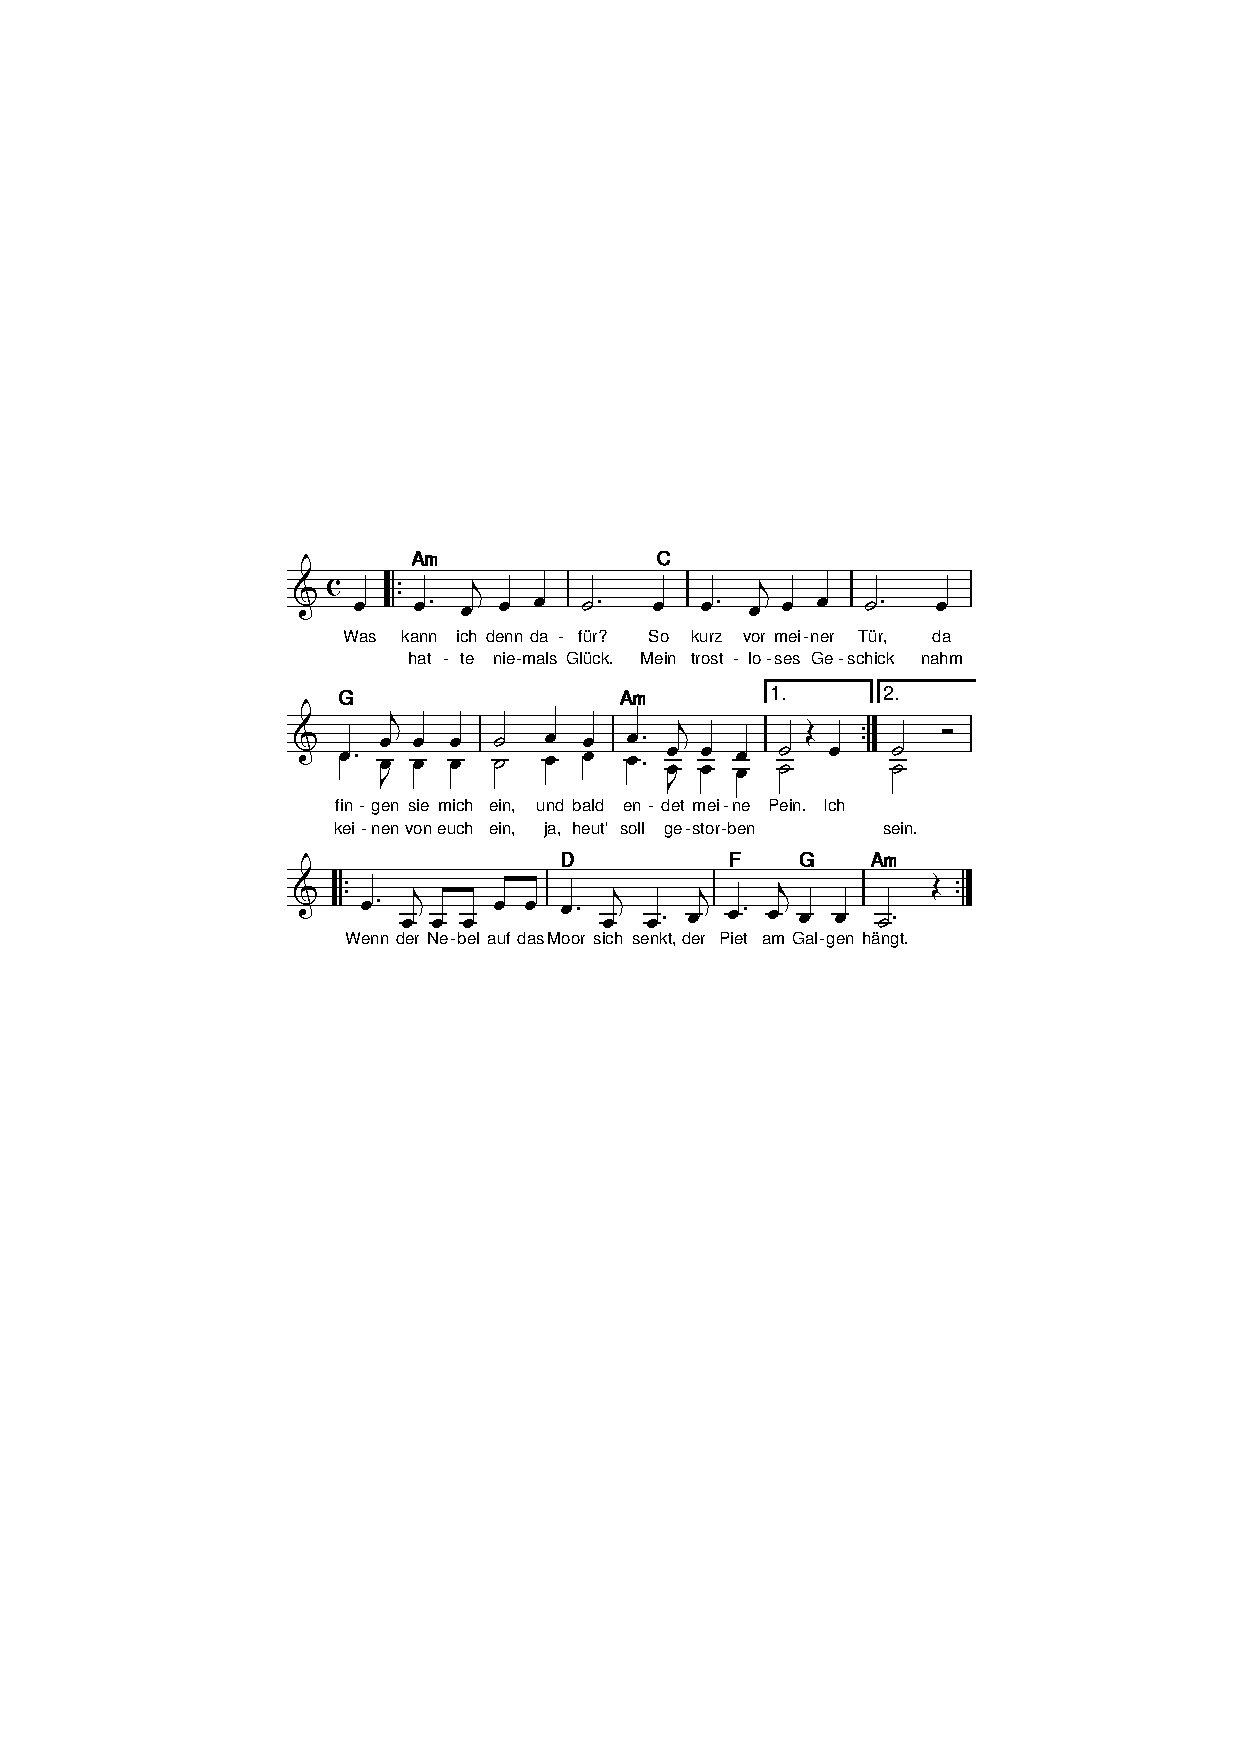
\includegraphics{Noten/DerPiet.pdf}	

\beginverse

Was \[Am]kann ich denn dafür? So \[C]kurz vor meiner Tür 
da \[G]fingen Sie mich ein und bald \[Am]endet meine Pein.
Ich \[Am]hatte niemals Glück. Mein \[C]trostloses Geschick 
nahm \[G]keinen von Euch ein. Ja, heut \[Am]soll gestorben sein.
\endverse

\beginchorus
\lrep \[Am]Wenn der Nebel auf das \[D]Moor sich senkt, der \[F]Piet am \[G]Galgen \[Am]hängt.\rrep
\endchorus

\beginverse
Sie ^nahmen mir die Schuh' und ^auch den Rock dazu.
Sie ^banden mir die Händ und mein ^Haus, es hat gebrennt. 
Ich ^sah den Galgen steh'n. Sie ^zwangen mich zu gehn. 
Sie ^wollten meinen Tod, keiner ^half mir in der Not.
\endverse

\beginverse
Was ^kratzt da am Genick? Ich ^spür den rauhen Strick.
Ein Mönch der betet dort und spricht ^für mich fromme Wort;
die Wort, die ich nicht kenn, wer ^lehrte sie mich denn? 
Fünf ^Raben fliegen her, doch ich ^sehe sie nicht mehr.
\endverse
\endsong

\beginscripture

Lorem ipsum dolor sit amet, consetetur sadipscing elitr, sed diam nonumy eirmod tempor invidunt ut labore et dolore magna aliquyam erat, sed diam voluptua. At vero eos et accusam et justo duo dolores et ea rebum. Stet clita kasd gubergren

\endscripture

\begin{intersong}
\centering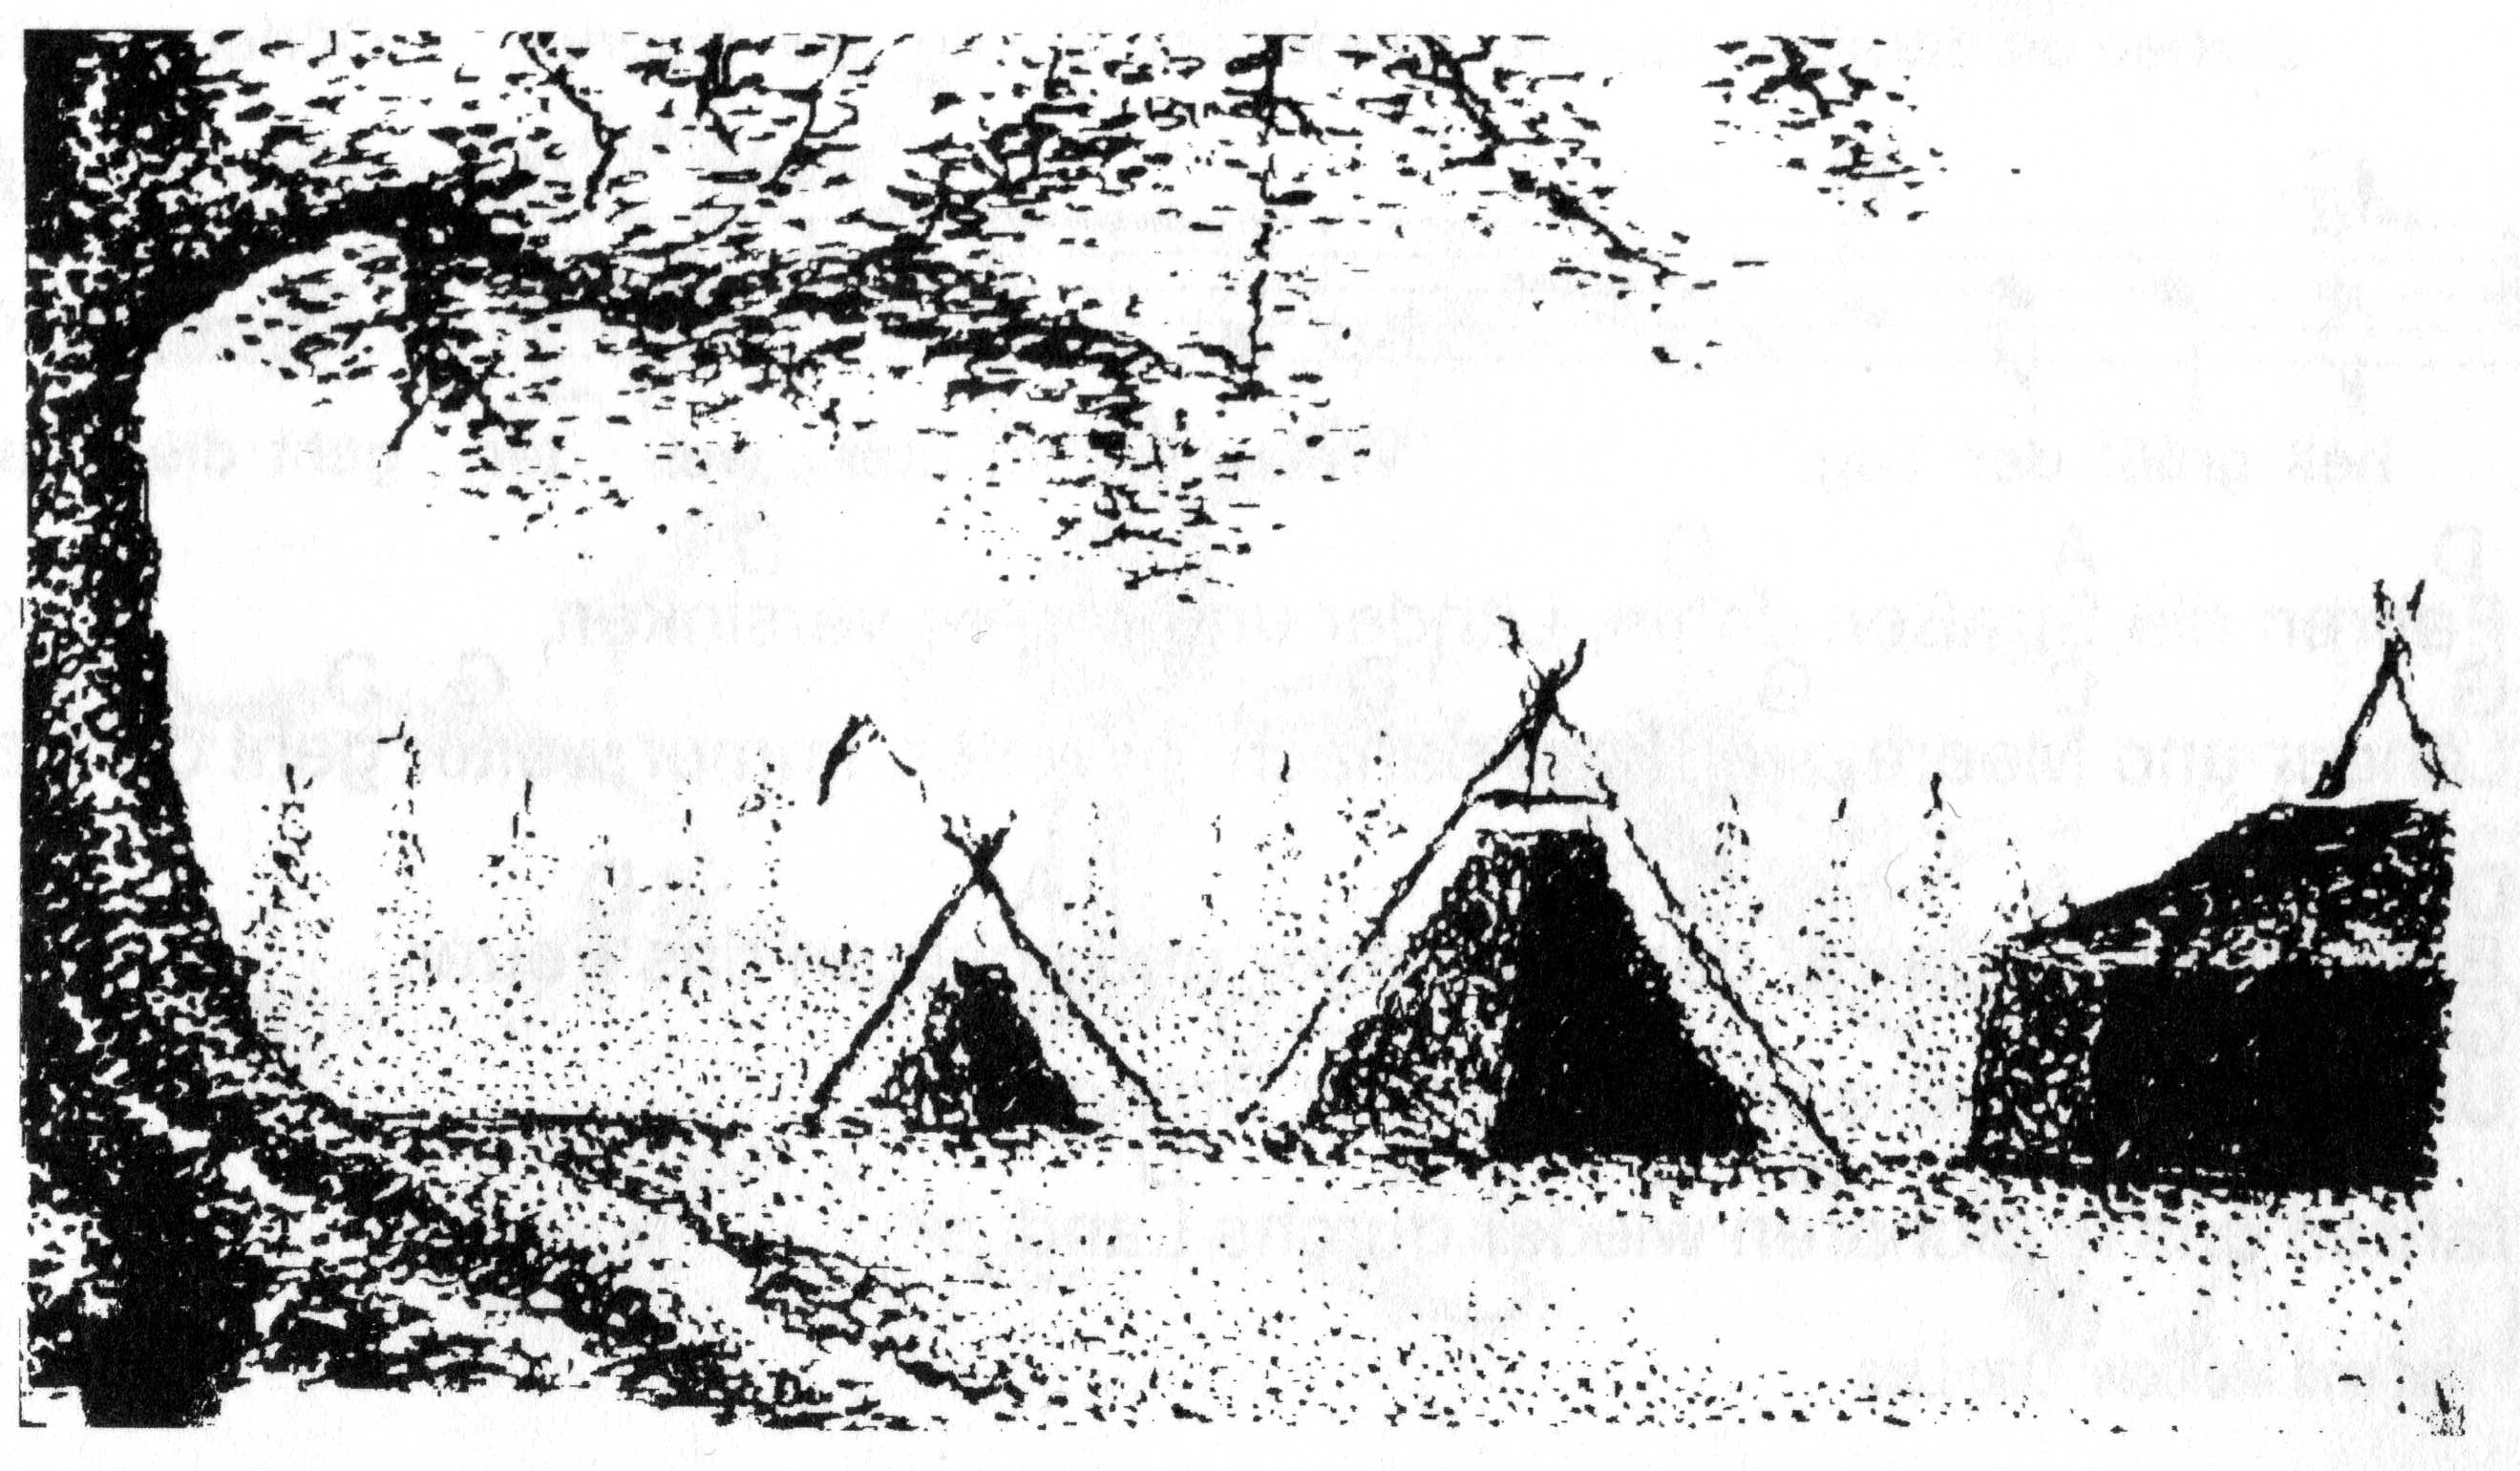
\includegraphics{Bilder/lager001.jpg}
\end{intersong}